\chapter{Energy Reconstruction}
\label{chap:Energy Reco}

\section{Pandora/Larsoft Overview?}

Use vertex sample - make life easier for Pandora.

\begin{itemize}
    \item Current induced on wires.
    \item Extract signal from noise and e-field etc.
    \item some more stuff
    \item Pandora patter recognition clusters the reconstructed hits.
    \item Initially 2d clusters are made. Clusters are then matched between planes to produce 3d clusters
\end{itemize}

Patter recognition classifies particles as either track-like or shower-like. Naturally, the shower reconstruction tools are only run on the shower-like particles.




\section{Motivation for improving the shower energy reconstruction}
Important for the selections. 
Need to correct for SCE + explain SCE. Show non linear EField

The electric field in the \Glspl{tpc} are designed to be uniform between the \Gls{cpa} and the \Glspl{apa}, however, due to for example cosmic muons, argon atom may be ionised. The ionised electrons and argon ions then drift towards the anode and cathode respectively, however the drift time for the ions is much greater than the electron drift time. This results in a positive charge build up towards the cathode which in turn will pull the drifting electrons towards the \Gls{tpc} centre. This is known as the \Gls{sce} and causes the electric field in the \Gls{tpc} to be non-uniform. An example of the modified non-uniform electric field is shown in \FigureRef{fig:SCE_map}. Space charge is expected to be a non-negligible effect in SBND, therefore any shower reconstruction algorithms need to be able to correct for a recombination effect which is electric field dependent. This is further discussed in \SectionRef{subchap:shower reco overview}.

\begin{figure}[h]
    \centering
    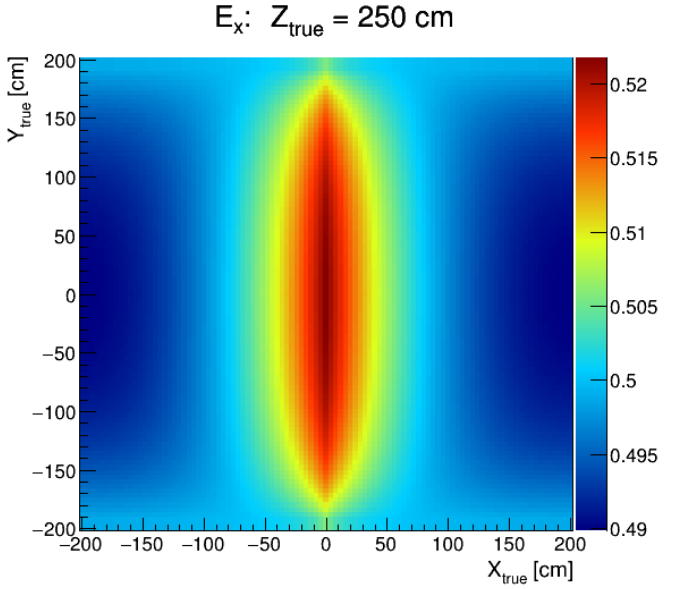
\includegraphics[width = \largefigwidth]{figures-chap4/SCE_map_SBND.png}
    \caption{The expected electric field offset relative to the nominal value of 0.5 kV/cm at z~=~250cm in SBND (the centre of the detector) caused by SCE.}
    \label{fig:SCE_map}
\end{figure}


\section{Overview of shower energy reconstruction in SBND}\label{subchap:shower reco overview}
Reconstructing shower energies predominantly involves calculating the charge collected by the \Gls{tpc} wire planes and estimating an associated energy. Detector dependant effects such as electron lifetime and recombination need to be accounted for. Electron lifetime is a measure of the free electrons lost due to attachment to impurities in the liquid argon whilst drifting across the detector \cite{ArgoNeuT_electron_lifetime_paper}. When argon atoms are ionised, the resulting argon ion and ionised electron may immediately recombine. This is known as the recombination effect and the magnitude of the effect is largely due to the local electric field \cite{ArgoNeuT_recombination_paper}. 

Correcting for the recombination effect directly is not straightforward because it is dependent on $\frac{dE}{dx}$ (see \EquationRef{eqn:ModBox} and unlike for track-like objects, reconstructing the 3D trajectory for showers is difficult \cite{MicroBooNE_photon_Ereco_paper}. Two different approaches have been considered and are discussed in the relevant energy reconstruction methods below; 1) Assume a nominal recombination value for all hits and 2) use a lookup curve which relates the collected charge to energy which circumvents the need to evaluate a recombination correction because it is already accounted for in the curve.

\subsection{Linear Energy Tool}\label{subchap:Linear Energy Tool}
The first shower energy reconstruction method developed as part of the \textit{PandoraShower} suite of tools was the \textit{Shower Linear Energy tool}. This tool relies on the linear relationship between the true energy deposited in the detector and the reconstructed charge. A sample of \Gls{mc} muons are used as calibration because the $\frac{dE}{dx}$ value for electrons and \Gls{mip} muons are not dissimilar. The relationship between the charge obtained from the hits due to the muons and the energy deposited by the muons is shown in \FigureRef{fig:linear lookup curve}. A linear relationship such as this is comparable to assuming a constant recombination factor. 



%\begin{center}
%    \centering
%    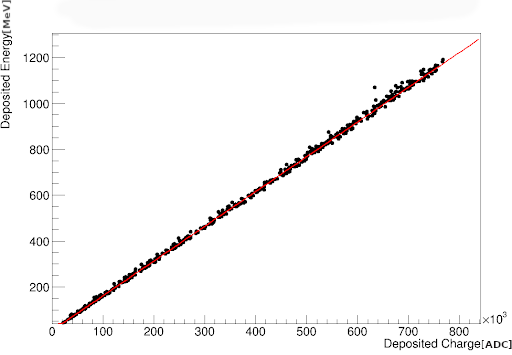
\includegraphics[width = 0.7\textwidth]{figures-chap4/linear_energy_lookup_curve1.png}
%    \captionsetup{type=figure}
%    \captionof{figure}{The linear relationship between deposited charge and energy. Produced from a sample of muons used for calibrating the \textit{Shower Linear Energy tool.}}
%    \label{fig:linear lookup curve}
%\end{center}
\newpage
\begin{figure}[h]
    \centering
    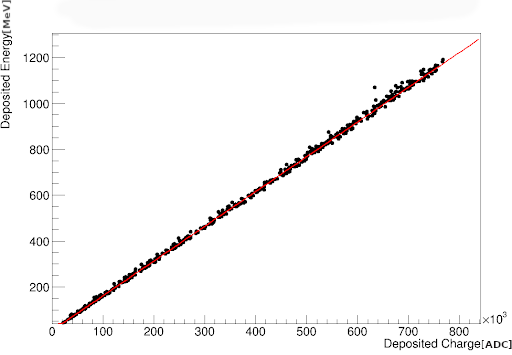
\includegraphics[width = \largefigwidth]{figures-chap4/linear_energy_lookup_curve1.png}
    \caption{The linear relationship between deposited charge and energy. Produced from a sample of muons used for calibrating the \textit{Shower Linear Energy tool.}}
    \label{fig:linear lookup curve}
\end{figure}



To estimate the reconstructed shower energy, the hits from the shower are found and integrated over to obtain the charge in \Gls{adc} units. The charge is corrected to account for electron lifetime and then the linear dependency is used to convert the charge to deposited energy. A further recombination correction is not required as it has already been accounted for in the charge to energy conversion. The fractional energy resolution of the \textit{Shower Linear Energy tool} is shown in \FigureRef{fig:linear_kGeVelectrons}. 

\subsection{Number of Electrons to Energy}\label{subchap:kGeVToElectrons}
The \textit{Shower Num Electrons Energy Tool} was developed to move away from being reliant on in-house calibration curves and instead use the pre-existing calibration available in the \Gls{sbnd} portion of the \Gls{larsoft} framework. The method to estimate the reconstructed energy is as follows; the charge for each hit is found and corrected for electron lifetime as is described in \SectionRef{subchap:Linear Energy Tool}, a correction for the recombination effect is applied, the charge is then converted to the number of electrons using the \Gls{sbnd} \textit{CalorimetryAlg} and finally the number of electrons are converted to energy by use of a \textit{GeVToElectrons} scale factor which is the inverse of the energy required to ionise and argon atom. The recombination correction is taken to be a constant value of 0.64 for all hits. (NEED REFERENCE). \FigureRef{fig:linear_kGeVelectrons} compares the reconstructed energy from \textit{Shower Num Electrons Energy Tool} to the true energy of the showering electrons alongside the same results from the \textit{Shower Linear Energy tool}.

\newpage
\begin{figure}[h]
    \centering
    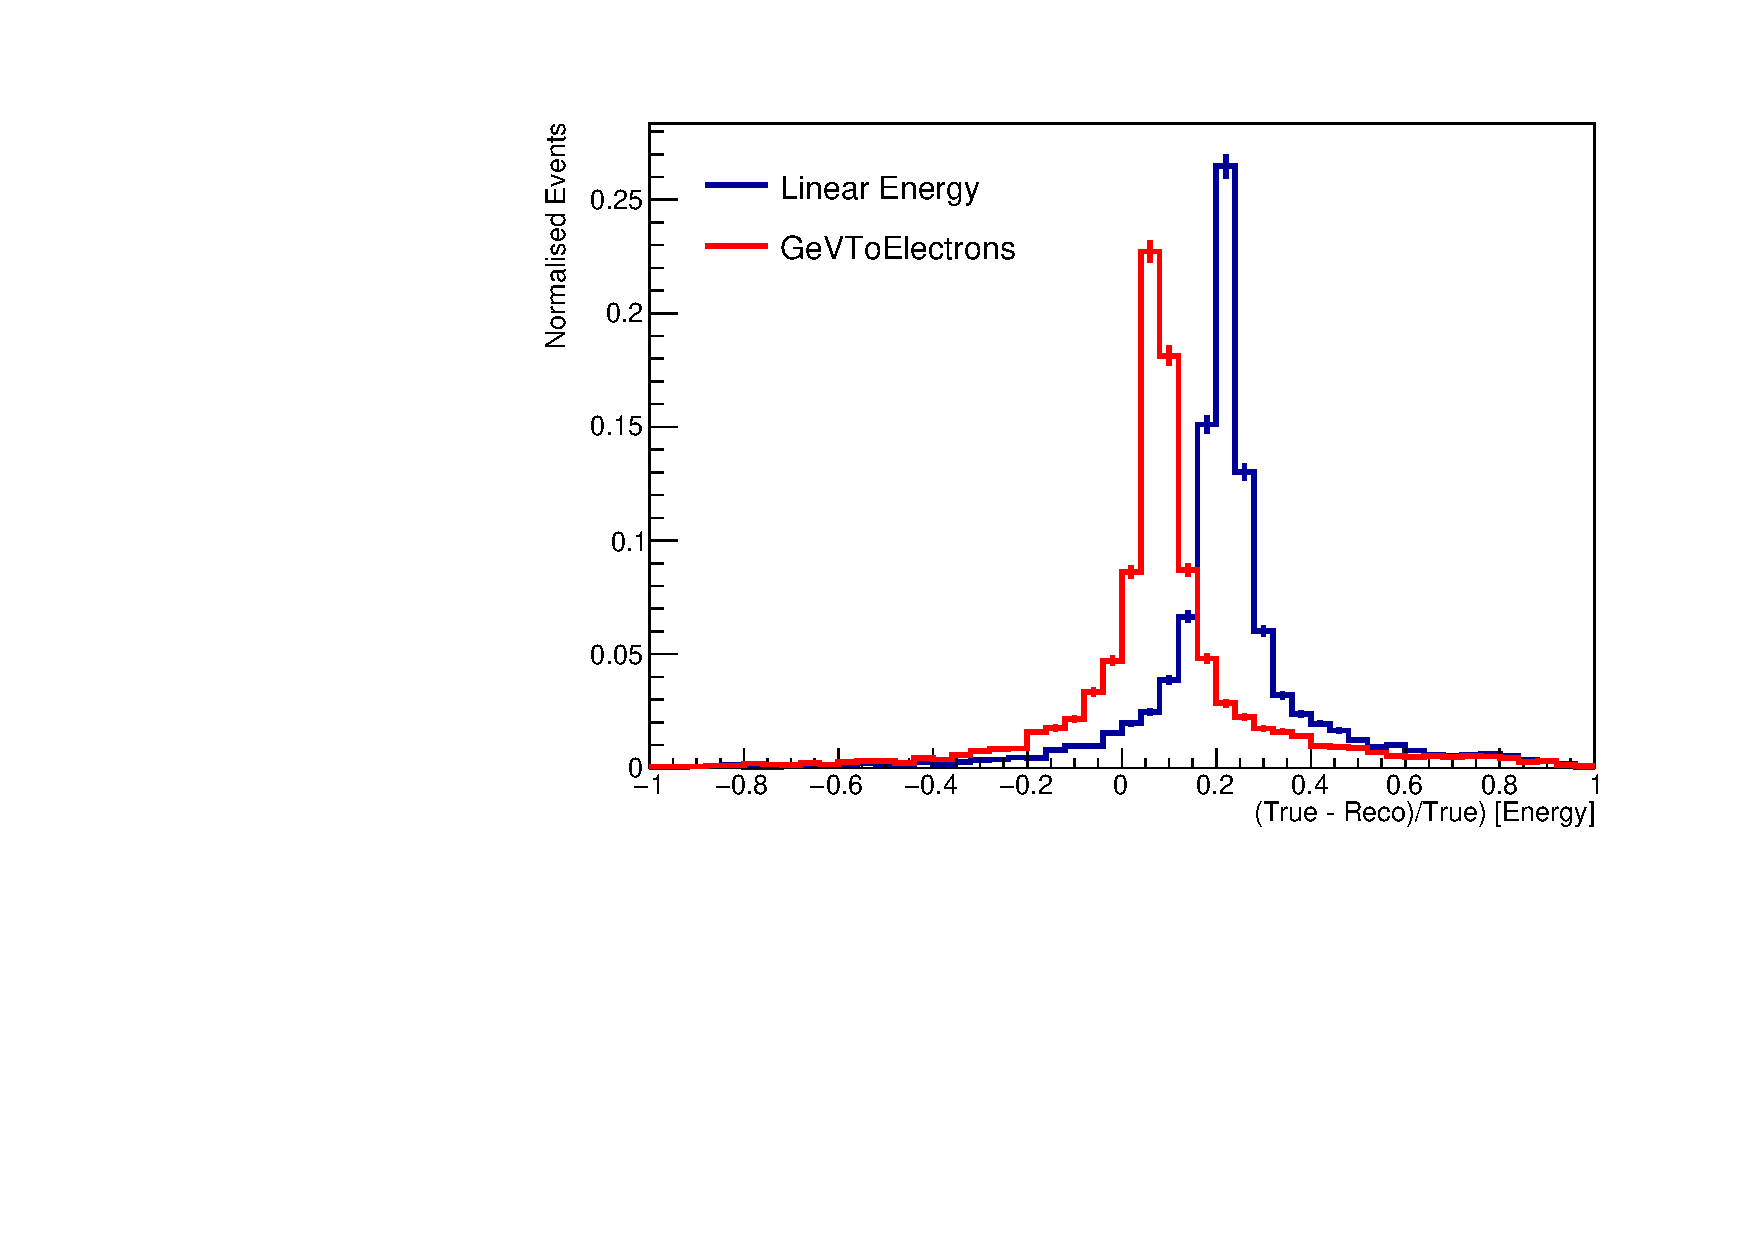
\includegraphics[width = \largefigwidth]{figures-chap4/linear_energy_kGeVElectrons_true_showering.pdf}
    \caption{Comparison of the \textit{Shower Linear Energy Tool} (Blue) and the \textit{Shower Num Electrons Energy Tool} (Red) with the true energy of the showering electrons.}
    \label{fig:linear_kGeVelectrons}
\end{figure}

An attempt to correct for the \Gls{sce} can be made with this method by utilising the Modified Box Recombination Model which is given by \begin{equation}\label{eqn:ModBox}
    \frac{dE}{dx} = \frac{\exp{(\frac{\beta}{\rho \mathcal{E}} W_{ion}.\frac{dQ}{dx}}) - \alpha}{\frac{\beta}{\rho \mathcal{E}}}
\end{equation}
where $\frac{dE}{dx}$ is the deposited energy per unit length, $\frac{dQ}{dx}$ is the deposited charge per unit length,  $\mathcal{E}$ is the electric field in the detector, $\rho$ is the density of liquid argon, $W_{ion} = 23.6$ eV which is the energy required to ionise an argon atom, $\alpha = 0.93 \pm 0.02$ and $\beta = 0.212 \pm 0.002$ (kV/cm)(g/cm$^2$)/MeV. The values for parameters $\alpha$ and $\beta$ are results from the \Gls{argoneut} experiment \cite{ArgoNeuT_recombination_paper}. The recombination correction, \textit{R} is given by $\frac{\frac{dQ}{dx}.W_{ion}}{\frac{dE}{dx}}$ and by taking the nominal values of \textit{R} and $\mathcal{E}$ a nominal value for $\frac{dE}{dx}$ is calculated using \EquationRef{eqn:ModBox}. Assuming the nominal value of $\frac{dE}{dx}$ is constant, \textit{R} may be expressed as $R = R(\mathcal{E}$). For each of the hits, their corresponding \Gls{sp} are found and the coordinates of the \Gls{sp} in the detector are determined. Instead of using the nominal value for $\mathcal{E}$, the local value for $\mathcal{E}$ at the position of the \Gls{sp} is used and the corresponding value for \textit{R} is calculated. The method to estimate the reconstructed energy is the same as the case without any \Gls{sce} corrections except the modified value for \textit{R} is used. In the case that a hit has no corresponding \Gls{sp}, the charge weighted centre of the shower is found and the local value of $\mathcal{E}$ at this point is used instead.

\begin{figure}[h]
    \centering
    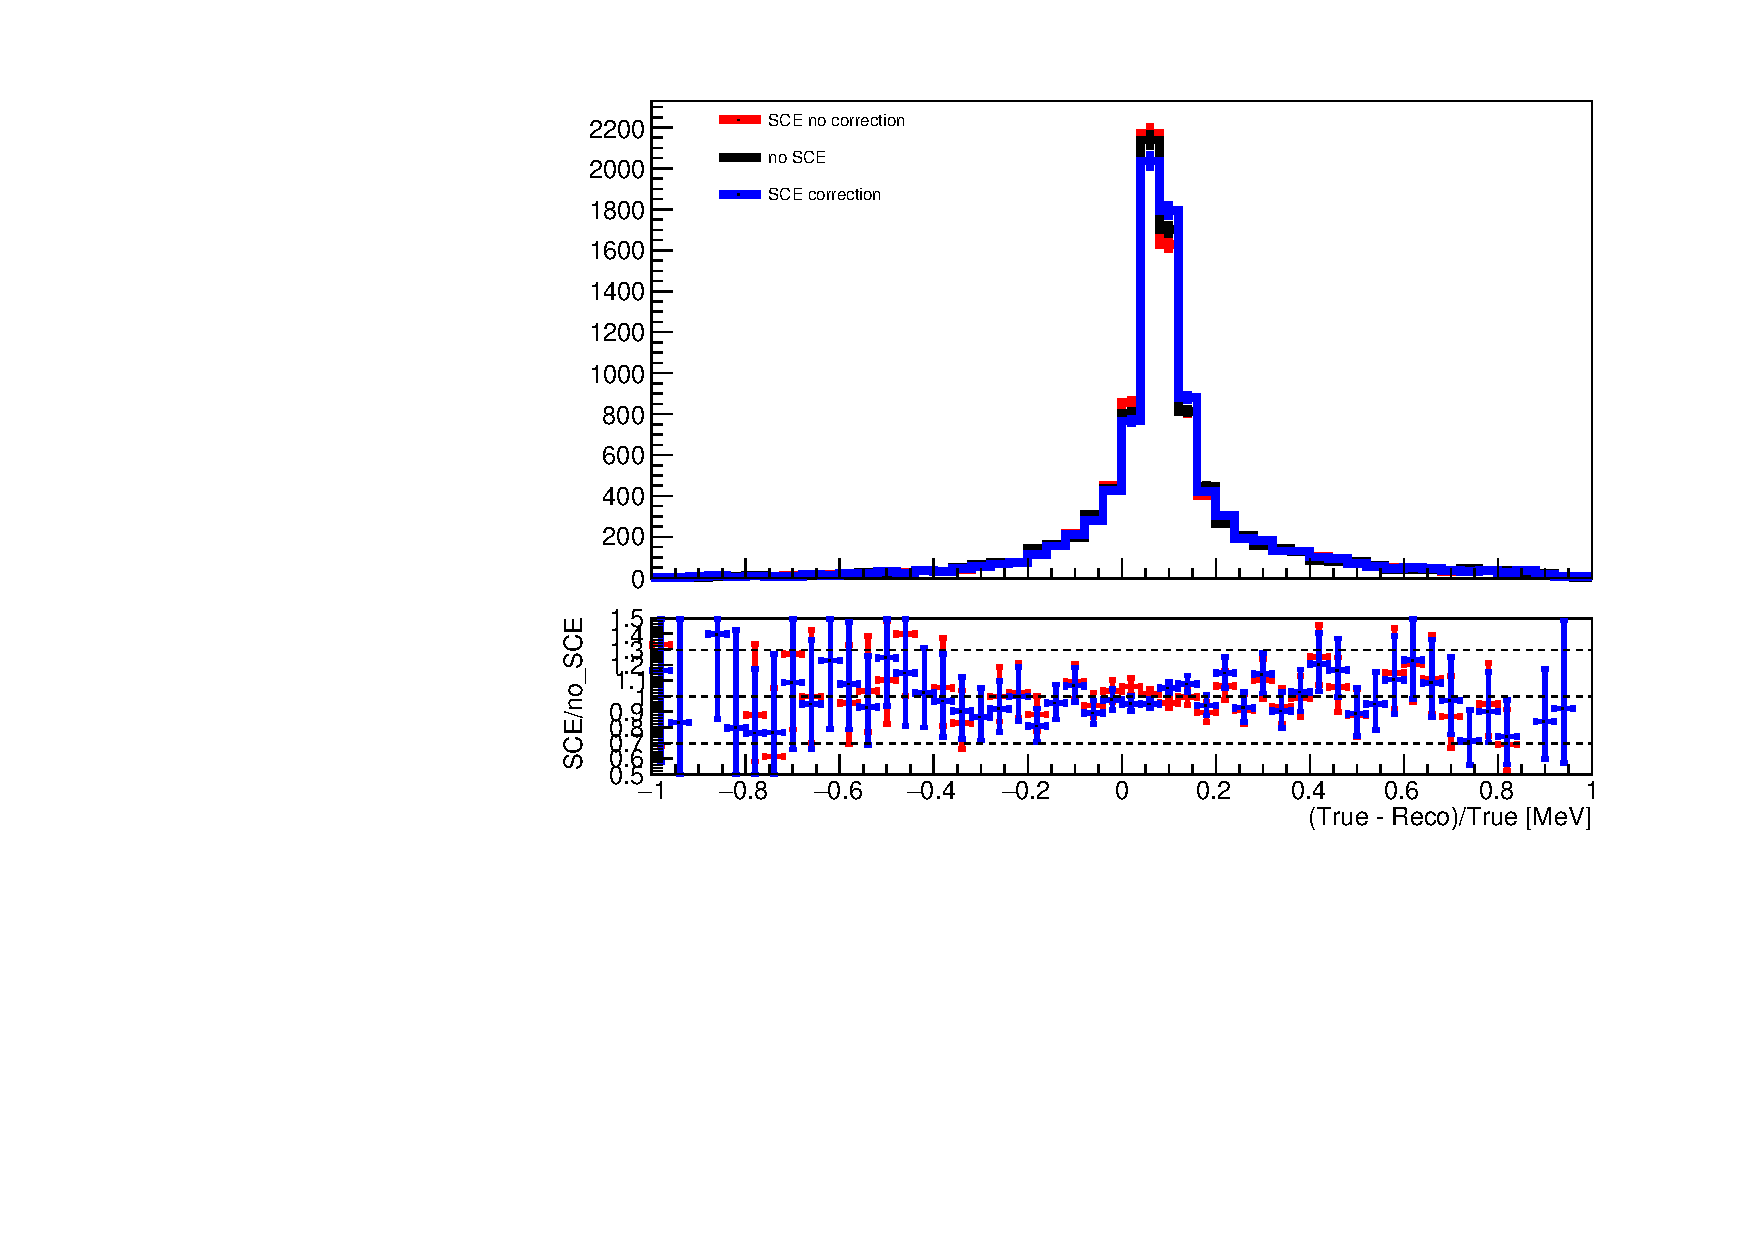
\includegraphics[width = \largefigwidth]{figures-chap4/ratio_plot_oldmethod_trueshoweringparticle.pdf}
    \caption{Caption}
    \label{fig:my_label}
\end{figure}



Shortcoming (don't know how much to put here? don't know if i want to emphasise how bad stuff is..): 
\begin{itemize}
    \item Things revolve around the nominal recomb of 0.64 - not really that realistic. 
    \item Correcting for SCE 'properly' is not straightforward either - using a fixed nominal dE/dx isn't ideal.
\end{itemize}

\section{Current method (ESTAR)}
The \textit{Shower ESTAR Energy tool} is the currently used method to reconstruct shower energy in SBND. It combines the ESTAR database along with the Modified Box recombination model. This approach was first used in the in \Gls{argoneut} experiment \cite{ArgoNeuT_ESTAR_paper}. The ESTAR database is provided by the \Gls{nist} and gives the track length of electrons in liquid argon for energies ranging from 0.01 MeV to 1000 MeV \cite{ESTAR_Database}.

The $\frac{dE}{dx}$ values are calculated by dividing the energy by the track length for each entry in the ESTAR database. The deposited charge, Q, is then found by using \EquationRef{eqn:ModBox} to find $\frac{dQ}{dx}$ and multiplying by the track length, dx. This now allows the deposited charge and energy to be related. If $\mathcal{E}$ in \EquationRef{eqn:ModBox} is taken to be a variable, the above process is repeated whilst iterating over a set values of $\mathcal{E}$. This results in a 3D curve relating both the deposited charge and electric field to energy as is shown in \FigureRef{fig:ESTAR lookup curve}. The overall reconstruction chain is similar to that described in \SectionRef{subchap:kGeVToElectrons}, but instead of directly converting the number of electrons using a scale factor, this lookup curve is used the interpolate the energy from the deposited charge and electric field. Electron lifetime corrections are applied as before, however a direct recombination correction is not required as this has been accounted for in the lookup curve. 

\begin{figure}[h]
    \centering
    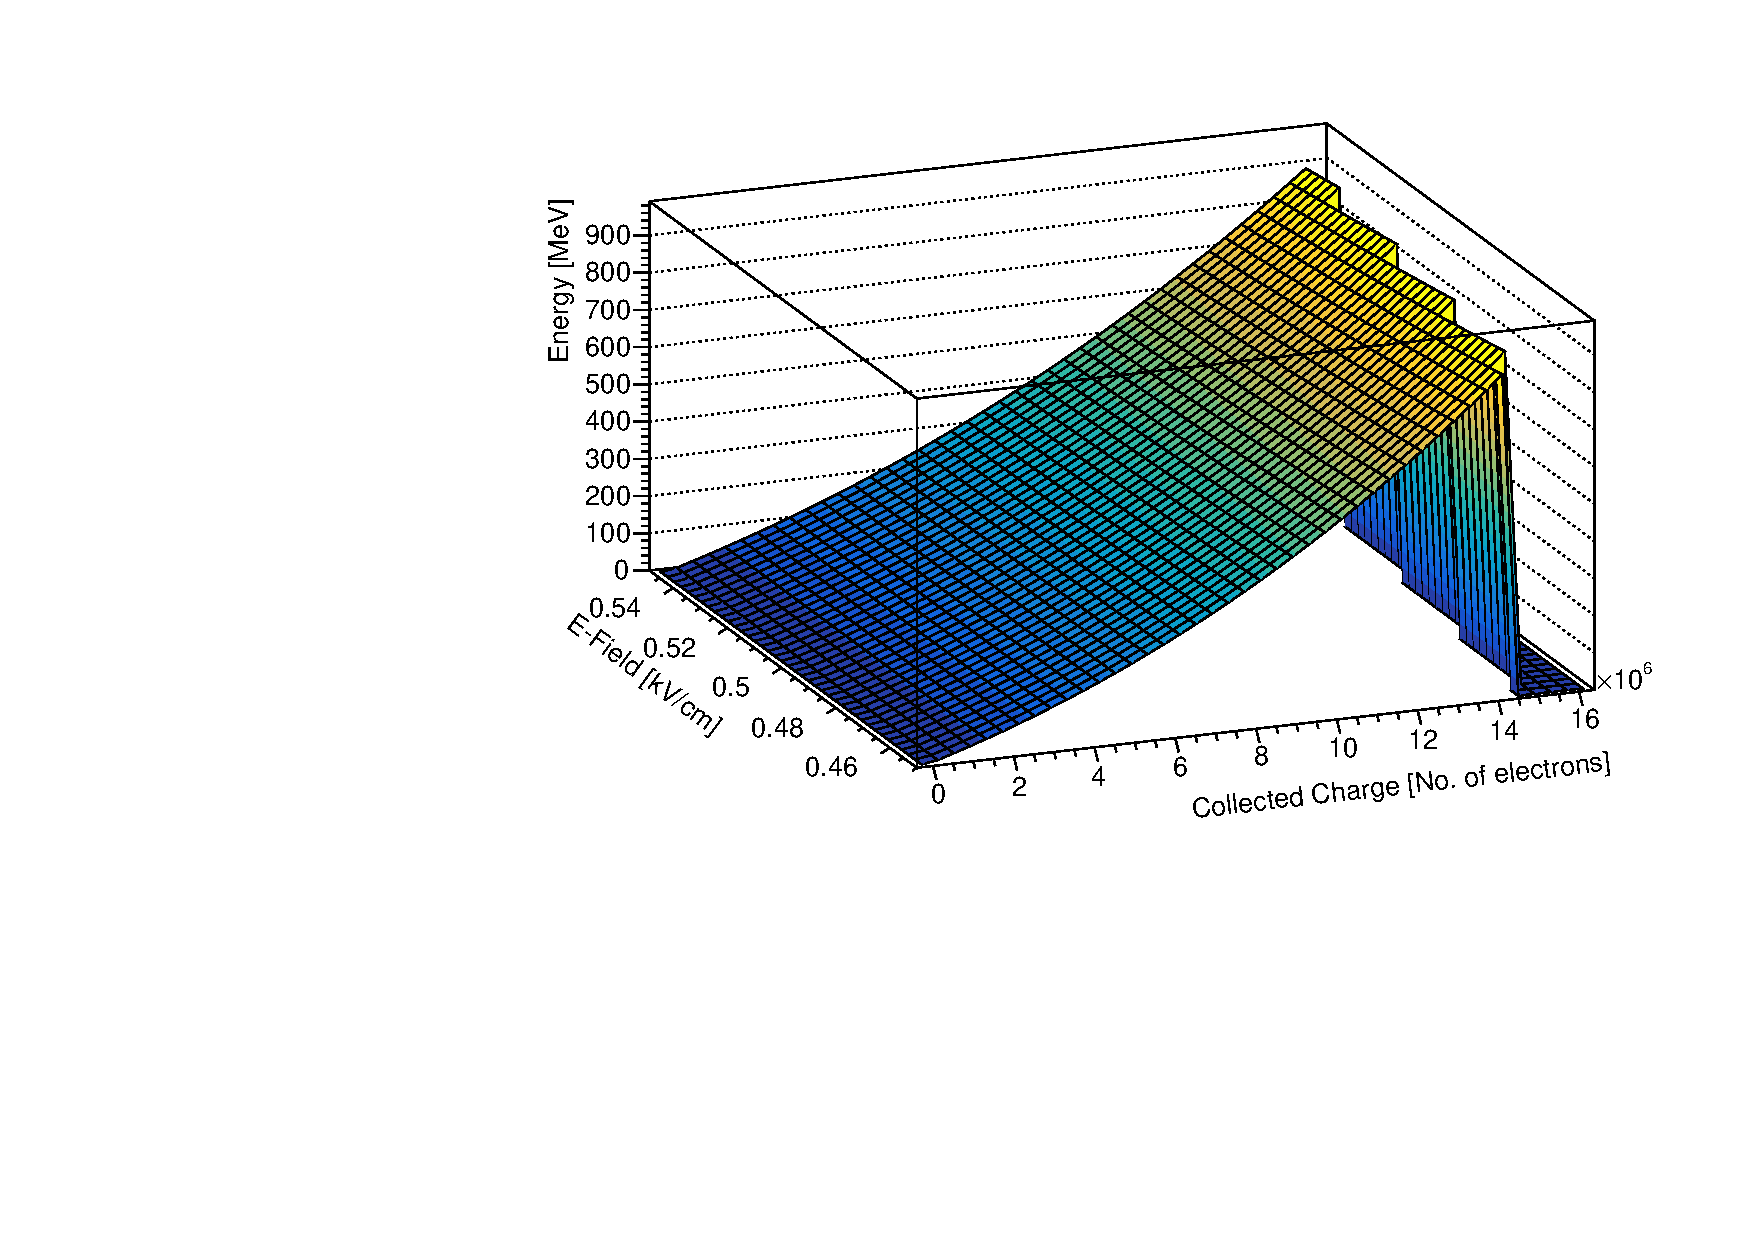
\includegraphics[width = 0.8\textwidth]{figures-chap4/ESTAR_lookup_curve.pdf}
    \caption{ESTAR Lookup Curve}
    \label{fig:ESTAR lookup curve}
\end{figure}

To assess the performance of the \textit{Shower ESTAR Energy tool}, the the reconstructed energy of each hit was summed up for all the hits in a shower. This was compared the sum of the true energy of all the hits.


\begin{figure}
    \centering
    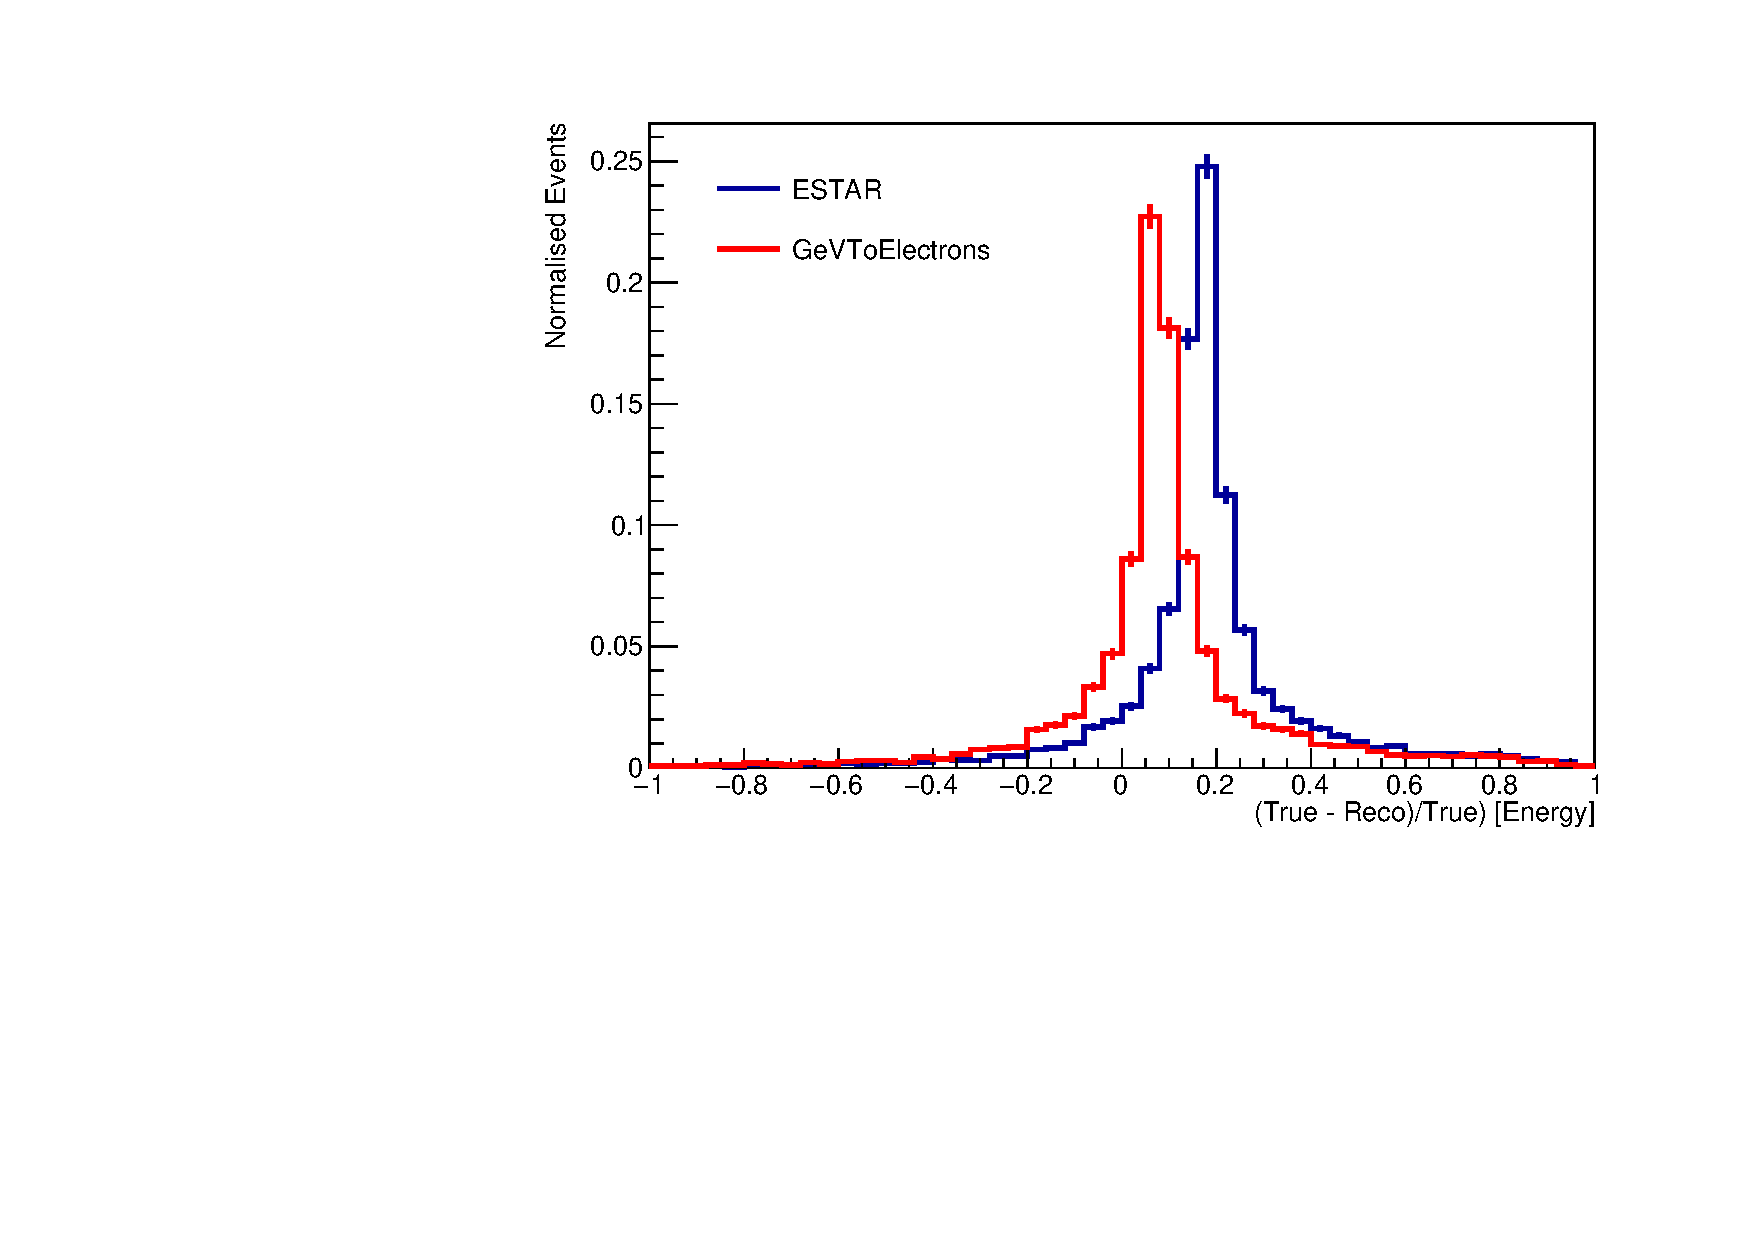
\includegraphics[width = \smallfigwidth]{figures-chap4/ESTAR_kGeVElectrons_true_showering.pdf}
    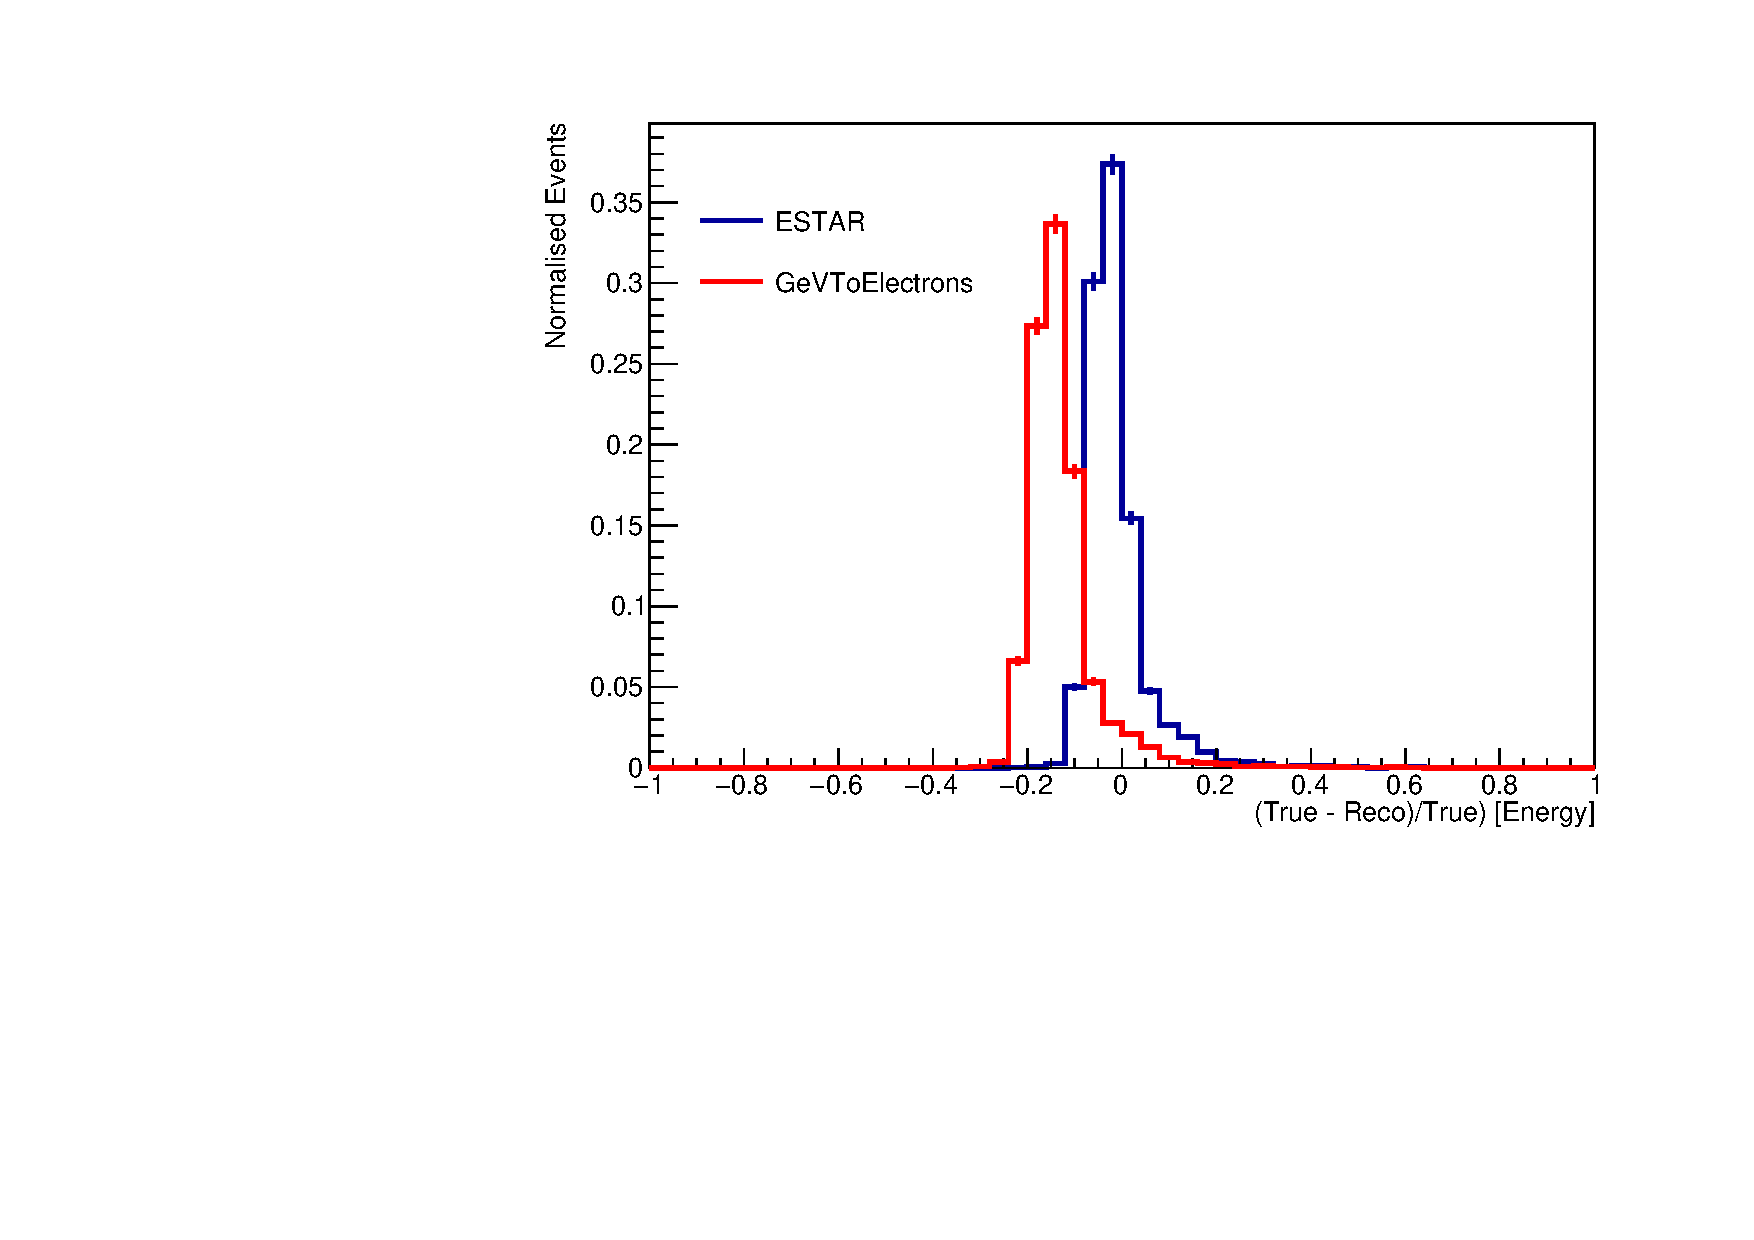
\includegraphics[width = \smallfigwidth]{figures-chap4/ESTAR_kGeVElectrons_true_hit.pdf}
    \caption{The fractional resolution of the \textit{Shower Num Electrons Energy Tool} and \textit{Shower ESTAR Energy Tool} compared with the true energy of the showering electron (left) and the sum of the true energy of all the hits (right). }
    \label{fig:my_label}
\end{figure}

\newpage
Other Validation stuff to do?
\begin{itemize}
    \item Use photon sample?
    \item validate for each individual plane and then best plane?
    \item Look at all showers in an event and compare with total showering energy. 
\end{itemize}


\section{Summary + outstanding issues etc}

Why getting dE/dx is hard (page 17).
Using muons as calibration
Energy bias corrections
https://inspirehep.net/files/f10063871db4836eb6ad935fcf761e7d

Energy Reco - Things to include.

\begin{itemize}
	\item Motivation (why do we care?)
	\item Explain choices - use vertex sample because it helps pandora. Only considering largest shower (most hits) from each event. 
	\item Overview of the very first method that was being used. Use muons to generate lookup curve. Get linear relationship between deposited charge and energy. Plagiarise Dom's thesis on this..  
	\item Change method so we convert the deposited charge to number of electrons and then convert the number of electrons to energy using the appropriate calibration/scale factors. Apply correction for electron lifetime as before and also correct for recombination. Previously recombination correction was 'baked' into the look-up curve. No way to correct for it directly - whenever we would change the \textit{physics} we would need to regenerate the look-up curve. With this method it's possible to tweak the recombination correction directly. 
	\item Not straight forward to calculate the recombination directly - let's use and average value for all showers - explain recombination study. 
	\item Consider SCE - explain what SC is.
	\item How do we account for SCE? Get map of the E-field in the detector (not uniform because of SC). Using the nominal value of the recombination and E-field, calculate a nominal dE/dx (not straightforward to calculate directly) which we assume remains constant. Can now use the Modified Box model to weak the recombination correction by feeding the local E-field (which depends on the location in the detector) back into the modified box model. Finally, find the (charge weighted) centre of the shower using the space points and use the local E-field at this point to calculate the recombination factor at this location. 
	\item No reason we can't do a per-hit analysis. Redo everything as before for each individual hit and then sum to get the energy of the shower. Should give better results since the recombination correction is more accurate now. 
	\item We have the ability to attempt to correct for the SCE as mentioned, but are limited by not knowing the dE/dx. So correcting the SCE without this caveat becomes tricky.. Try a new approach developed by ArgoNeuT - use the ESTAR database. The ESTAR database gives us the stopping power of (dE/dx) of electrons in various materials (including lAr) in a range of energies and is based partly from data. Combining this with the modified box recombination model, we can again create a lookup curve of energy vs deposited charge with the recombination correction baked in. Since the modified box model depends on the E-Field, we can treat this as a variable and create a 3D lookup curve of energy vs E-Field vs deposited charge which will allow us to correct for SC. 
	\item \textit{True} energy debacle.. We have the true energy of the showering particle and the true energy of all the hits in a given shower. Originally we used the true energy of the showering particle for comparison (in hindsight this seems like a stupid idea..) and the kGeVtoElectrons method clearly outperformed ESTAR. Swapping to the true hit energies, ESTAR does better. What was happening (i think) is that kGeVToElectrons over estimates the hit energies, so when comparing with the true showering particle this method give a better result because we're papering over the cracks due to the pattern recognition and hit inefficiencies. ESATR method gives a better result for individual hit energies so highlights the failing of the patter rec and hit inefficiencies when comparing with the showering particle. 
	\item Why some results are shit.. Pandora pattern recognition (clustering) is far from perfect - can use Pandora in cheating mode to overcome this. There are hit inefficiencies i.e. hit reconstruction isn't perfect - haven't ever \textit{cheated} this, dunno if it's an option. The actual impact from SC is pretty minimal but it also impacts Pandora's pattern recognition. This can a have a big impact - what Pandora initially recognised as one big shower may be interpreted as 2+ smaller showers after applying SC (and vice-versa). Also, an object classified as a shower may instead be classified as a track after applying SC. Since we're only considering the largest shower for each event, this effects mean SC can appear to have a impact. 
\end{itemize}
